%--------------------------------------------------------------------
%--------------------------------------------------------------------
% Formato para los talleres del curso de Métodos Computacionales
% Universidad de los Andes
%--------------------------------------------------------------------
%--------------------------------------------------------------------

\documentclass[11pt,letterpaper]{exam}
\usepackage[utf8]{inputenc}
\usepackage[spanish]{babel}
\usepackage{graphicx}
\usepackage{tabularx}
\usepackage[absolute]{textpos} % Para poner una imagen en posiciones arbitrarias
\usepackage{multirow}
\usepackage{float}
\usepackage{hyperref}
%\decimalpoint

\begin{document}
\begin{center}
{\Large Métodos Computacionales} \\
\textsc{Tarea 2}\\
01-2019\\
David Cartwright\\
\end{center}

\noindent
\section{Ejercicio 1: Fourier}
\subsection{subplots de señales sumadas e individuales} 
\begin{center}
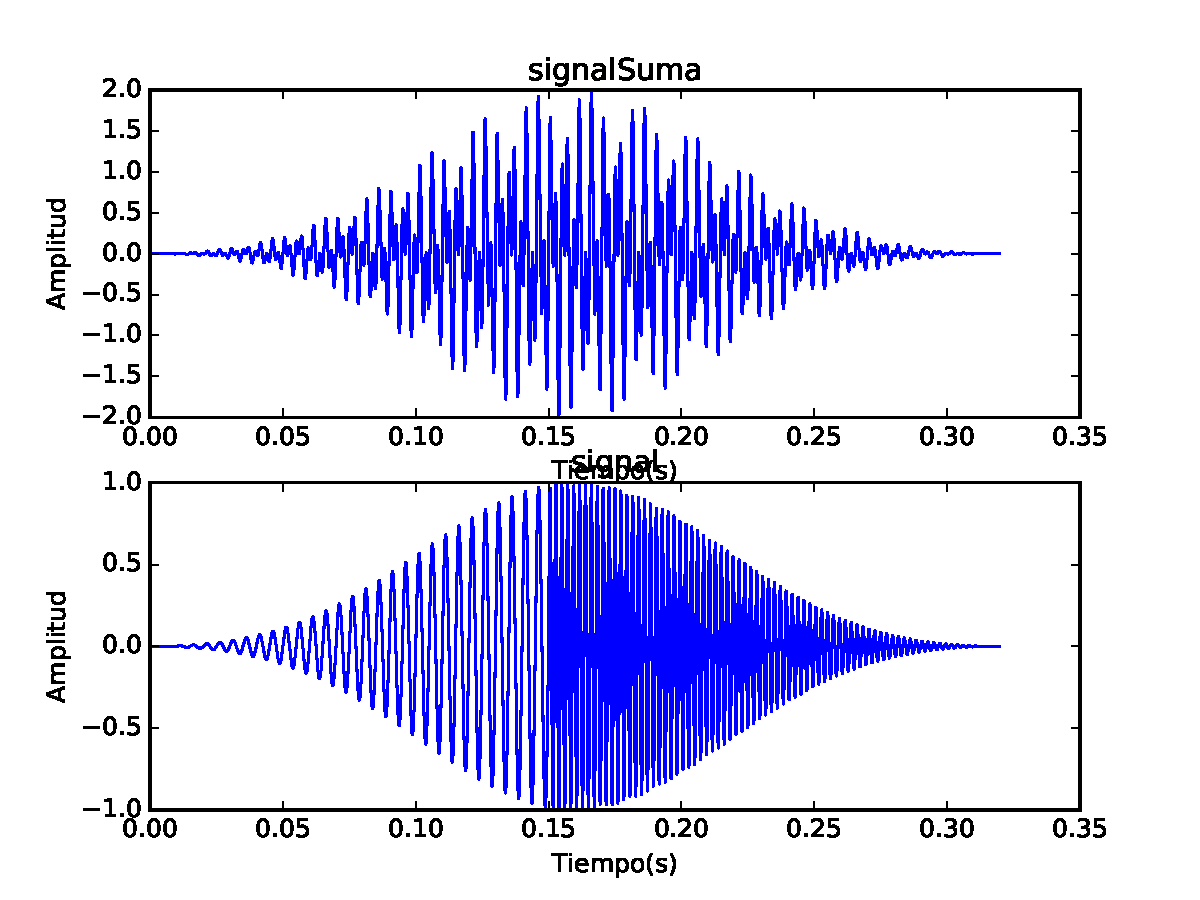
\includegraphics[width=10cm]{signal_subplots.pdf} 
\end{center}
En este grafico vemos representadas las señales sumadas en el plot superior y las individuales en el inferior. Se puede ver como varia la amplitud y la frecuencia, para el caso inferior, en el tiempo.

\subsection{Transormada de Fourier para las señales}
\begin{center}
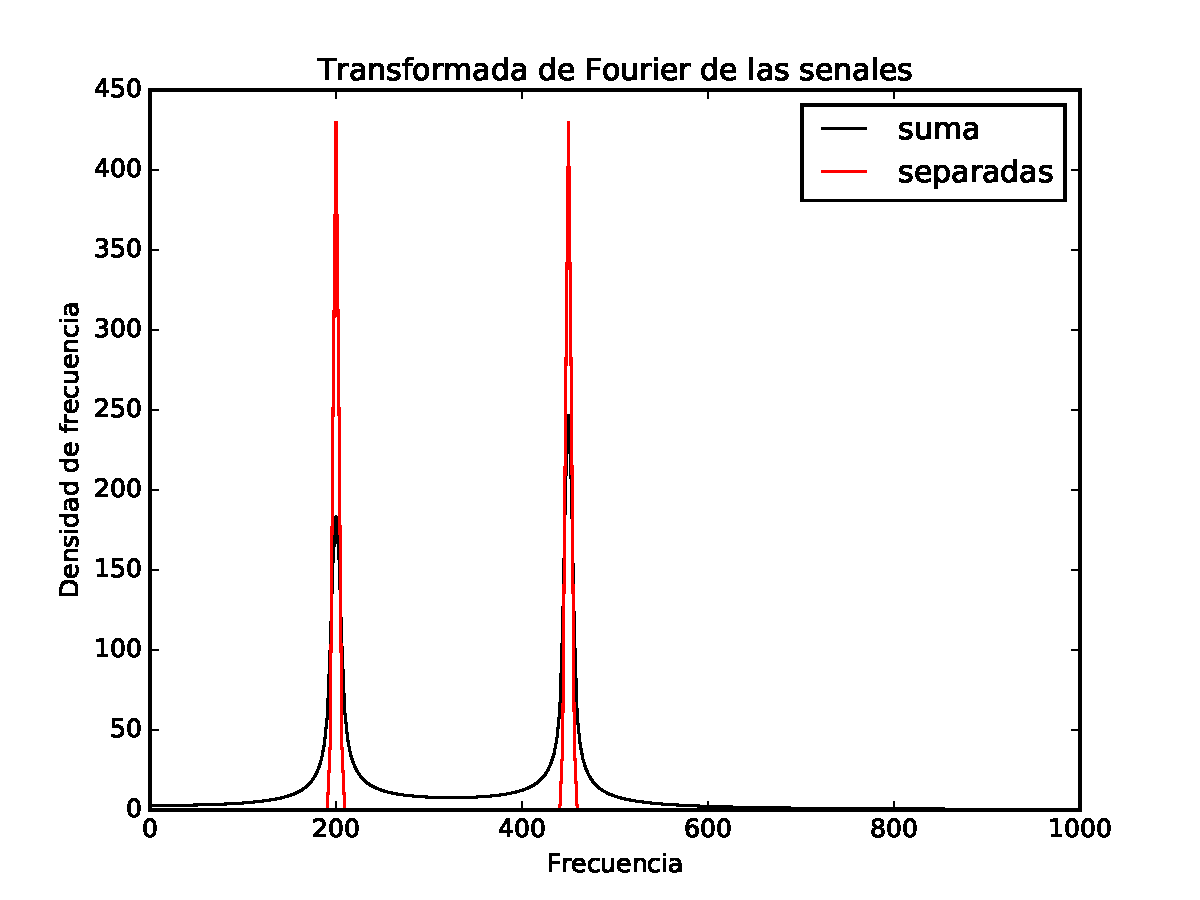
\includegraphics[width=10cm]{Fourier_senales.pdf} 
\end{center}
El grafico muestra la transformada de Fourier para ambas señales. Como se esperaba hay dos picos que indican los modos normales de cada señal, vemos que los picos de la suma son significativamente menores que los de las señales individuales.

\subsection{Espectrograma para las señales}
\begin{center}
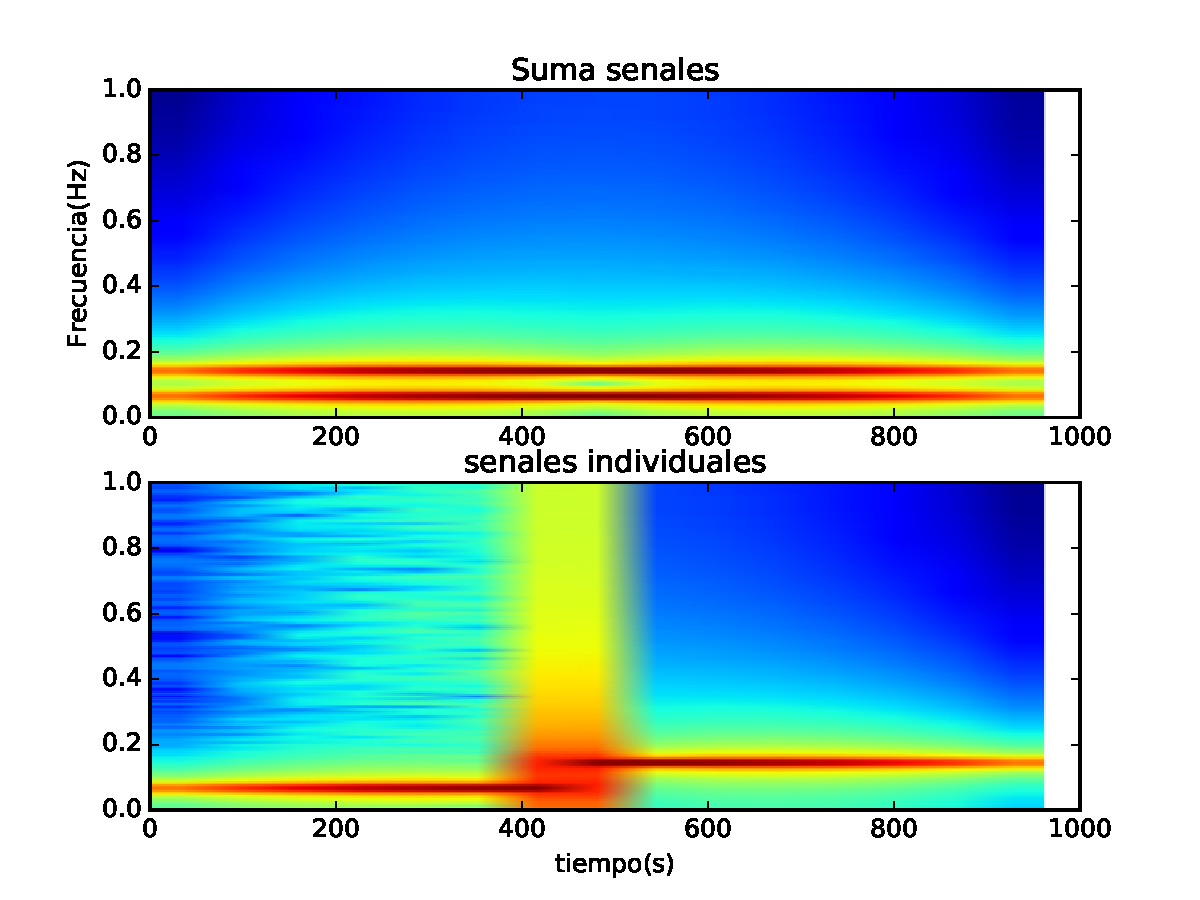
\includegraphics[width=10cm]{espectrogramas1.pdf} 
\end{center}
Los espectrogramas de las señales nos permiten visualizar mejor como estas se comportan, ya que en un grafico de 3 dimensiones podemos ver como la amplitud y la frecuencia se comportan en funcion del tiempo. En el grafico los colores rojos indican las mayores amplitudes, mientras que los azules/aguamarina indican las amplitudes mas pequeñas. Podemos ver que en el eje Y tenemos las frecuencias, por lo que vemos las lineas rojas paralelas al eje X indicando las frecuencias de los modos normales de estas señales. En el subplot de las señales individuales vemos una franja amarilla centrada, indicando el momento donde pasamos de la lectura de una señal a otra.

\subsection{Señal de un temblor real}
\begin{center}
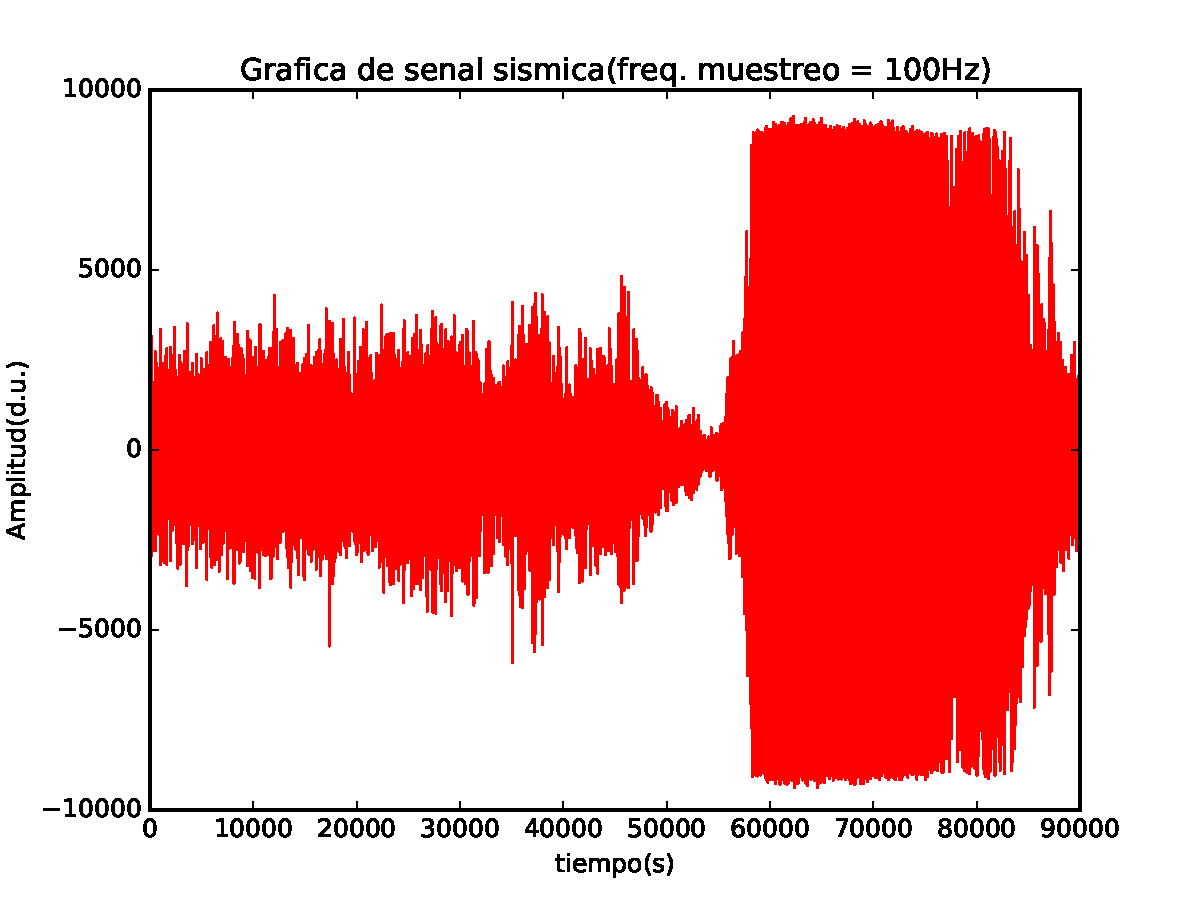
\includegraphics[width=10cm]{temblor.pdf} 
\end{center}
Este grafico es un sismograma de una señal de temblor real, podemos ver como comienza con una amplitud constante natural, posteriormente vemos como hay una disminucion de esta amplitud seguida de un drastico incremento de esta, lo que representa el comienzo del temblor.

\subsection{Transformada de Fourier señal de temblor}
\begin{center}
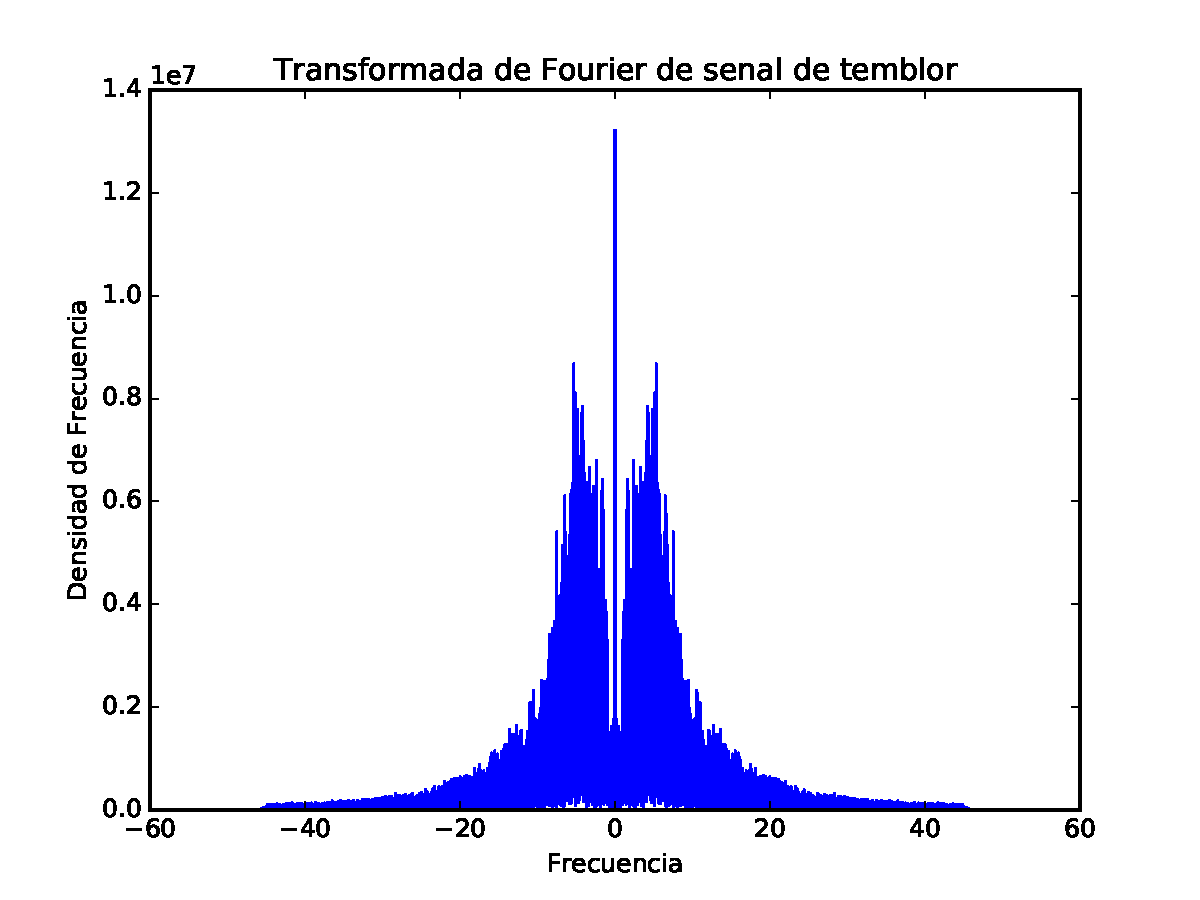
\includegraphics[width=10cm]{Fourier_temblor.pdf} 
\end{center}
La transformada de Fourier de la señal permite pasar al espacio de frecuencia representado en este grafico. En el grafico vemos que hay un pico alrededor de una frecuencia de 10Hz indicando el modo normal de esta señal.

\subsection{Espectrograma de señal de temblor}
\begin{center}
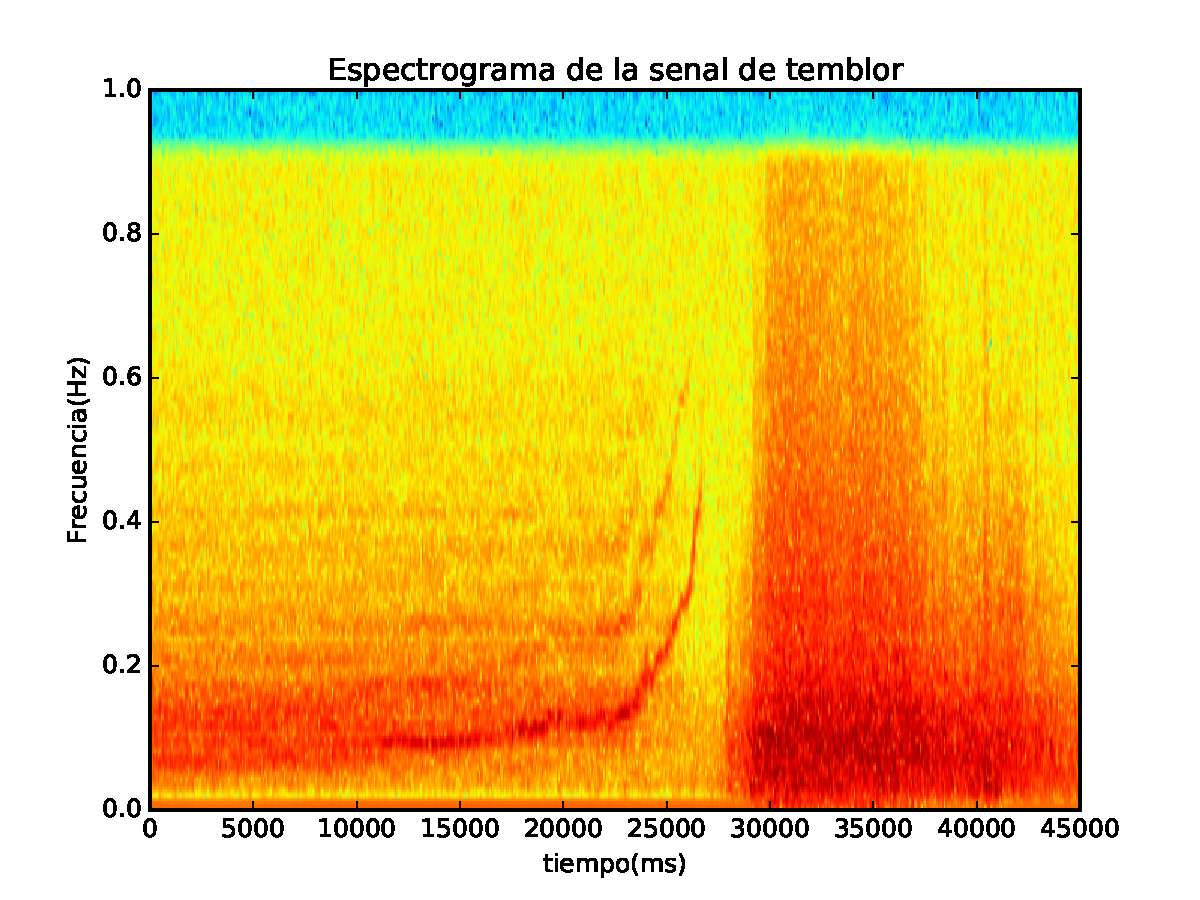
\includegraphics[width=10cm]{espec_temblor.pdf} 
\end{center}
Este es el espectrograma de la señal del temblor, como en el anterior los rojos son indicativos de amplitudes grandes mientras que los azules representan las mas pequeñas. La franja roja sobre 30000 en el eje X indica el momento donde inicia el temblor mostrando amplitudes bastante altas especialmente para las frecuencias mas bajas(<0.2). Podemos ver que antes de los 30000 milisegundos hay unas pequeñas curvas semi-horizontales de color rojo, estos pueden ser unos temblores precursores de menor magnitud, que aveces se registran previo a un sismo de mayor magnitud.

\section{Ejercicio 2: Ecuaciones diferenciales ordinarios: un edificio en un sismo}

\subsection{Amplitudes Maximas en funcion de la frecuencia}
\begin{center}
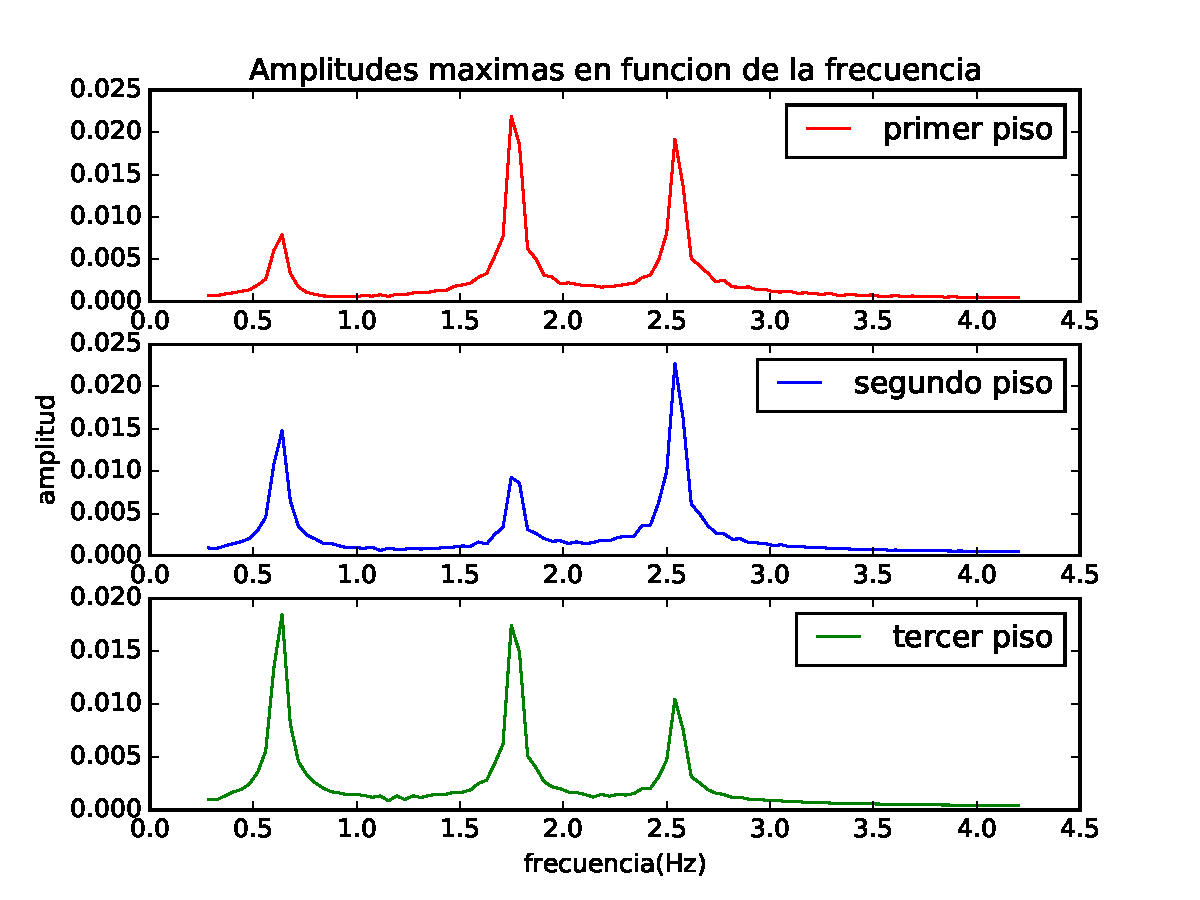
\includegraphics[width=10cm]{amp_max_edificio.pdf} 
\end{center}
En este grafico tenemos las amplitudes maximas en funcion de las frecuencias para cada piso. Podemos ver como el sismo afecta de manera diferente cada piso para una misma frecuencia. Para una frecuencia de 2.5 Hz tenemos una amplitud maxima cerca a 0.01 en el tercer piso, mientras que el segundo y el primer piso registran una amplitud de alrededor de 0.02; Por otro lado para una frecuencia cercana 0.67Hz vemos que el tercer piso tiene el valor mas alto(~0.018), mientras que el primer y segundo piso muestran valores menores que 0.015. Es interesante que para una frecuencia cercana a 1.75 Hz vemos una gran amplitud en el primer y tercer piso, mientras que el segundo muestra una amplitud un poco menor que 0.01, indicando que esa frecuencia haria menos daño en el piso intermedio que en los extremos. 

La mayor amplitud registrada se da en el segundo piso para una frecuencia cercana a los 2.6 Hz, esta probablemente es la frecuencia natural del edificio, ya que al coincidir la frecuencia del forzamiento(sismo) con la frecuencia natural se genera el efecto conocido como resonancia, donde se alcanzan los mayores valores de amplitud en el sistema. En este caso estamos modelando el edificio como un sistema de tres masas acopladas, por esta razon tenemos tres modos normales, cosa que se ve reflejada en los graficos como los tres picos en las amplitudes. Cada pico representa una de las frecuecias de los modos normales del sistema, donde se genera el efecto de resonancia y los pisos empiezan a desplazarse mucho mas generando los daños mas graves en la estructura.

\subsection{Graficos de amplitud en funcion del tiempo para los omegas elegidos}
\begin{center}
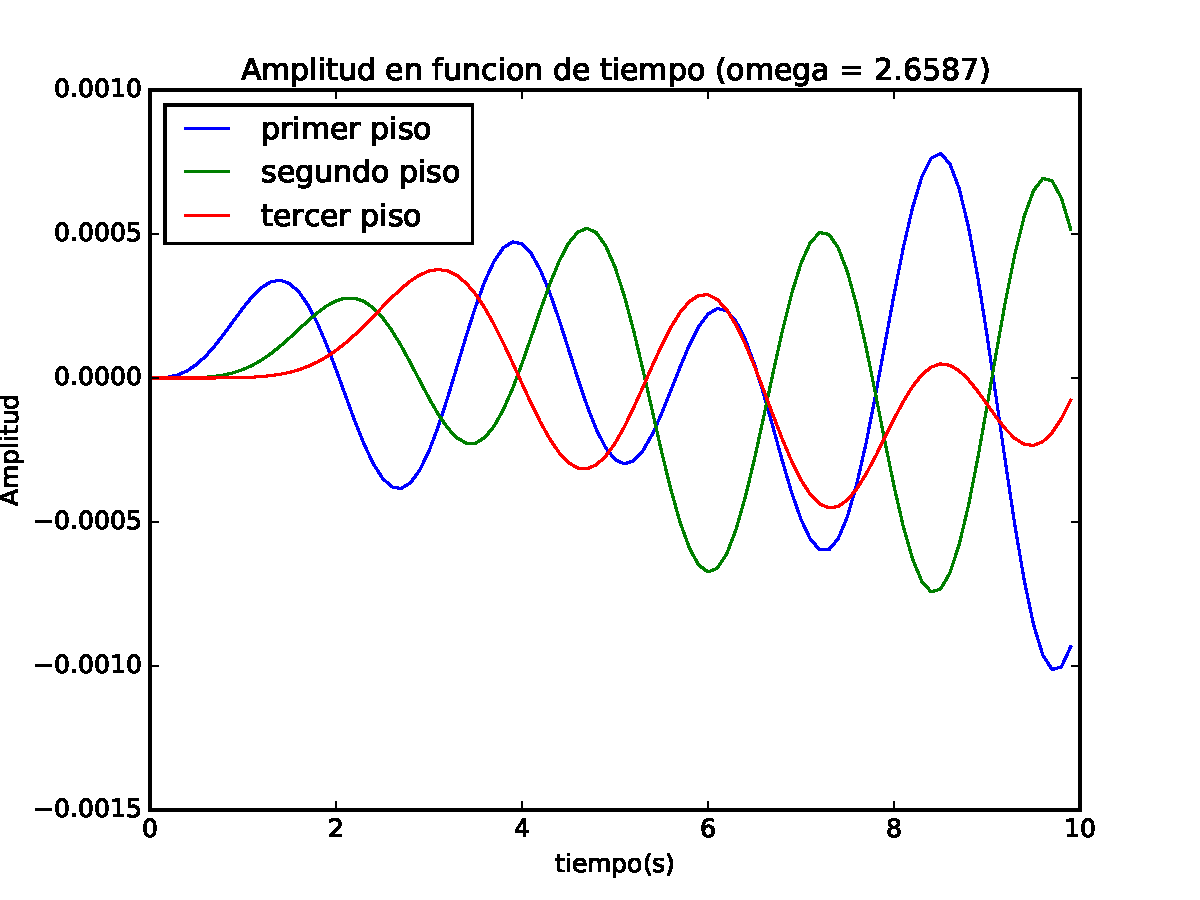
\includegraphics[width=10cm]{avst_o1.pdf} 
\end{center}  

El primer omega elegido tiene un valor de 2.6587 Hz, este fue elegido porque era muy cercano a uno de los modos normales del sistema, el que genero la amplitud de resonancia mas elevada. Como se vio en el grafico de las amplitudes maximas estos valores de frecuencia afectan en mayor proporcion a los pisos inferiores, en este grafico podemos ver como la curva de la amplitud para el tercer piso muestra unas amplitudes mucho menores que las de los pisos inferiores.
 

\begin{center}
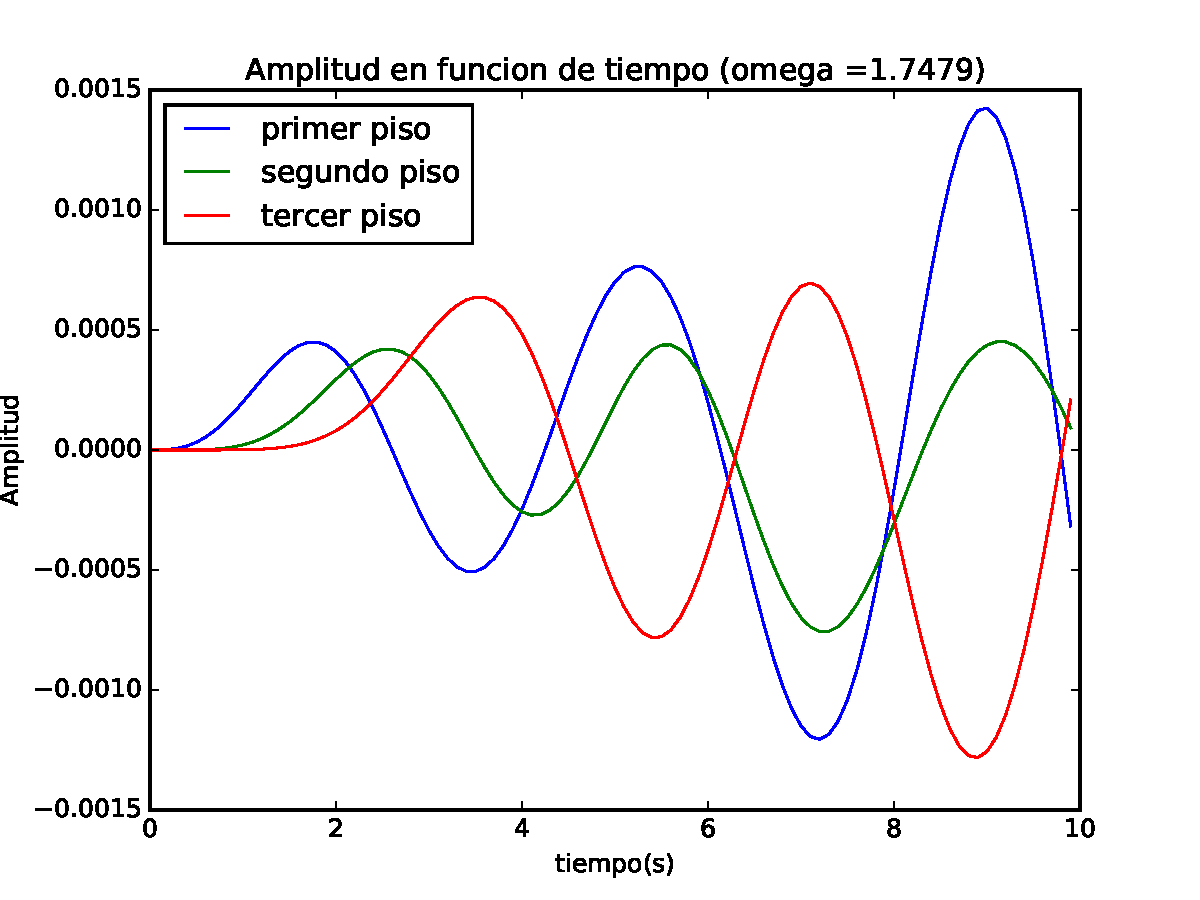
\includegraphics[width=10cm]{avst_o2.pdf} 
\end{center} 

El segundo omega tiene un valor de 1.7479 Hz, tambien elegido dada su cercania a uno de los modos, este nos permite ver el momento de resonancia donde el segundo piso es el menos afectado, mientras que el primer y tercer piso empiezan a tomar unas amplitudes mayores. 


\begin{center}
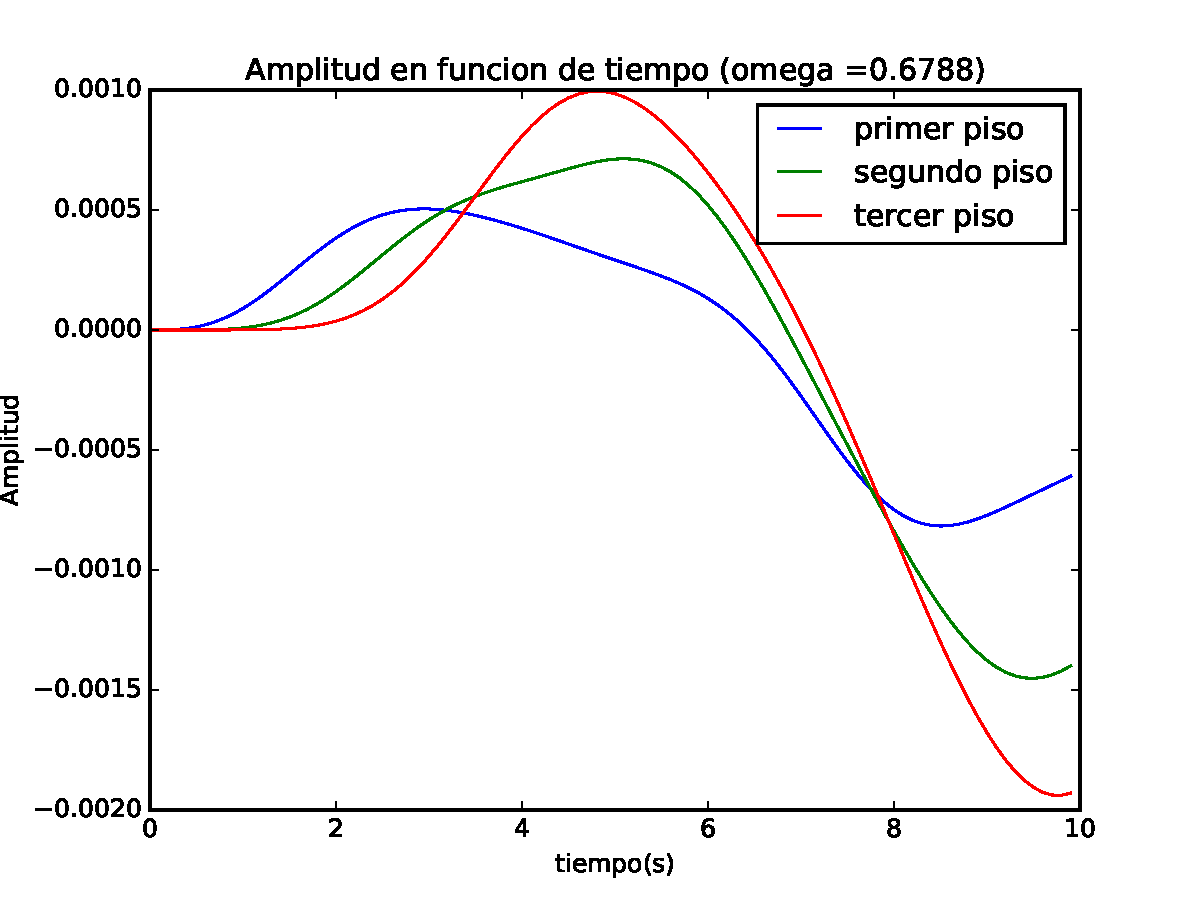
\includegraphics[width=10cm]{avst_o3.pdf} 
\end{center} 
El tercer omega tiene un valor de 0.6788 Hz y representa el tercer modo normal del sistema, en este caso como la frecuencia es tan baja no alcanzamos a ver un ciclo entero en el rango de tiempo de 10 segundos. Sin embargo se puede apreciar como el tercer piso es el que mas se desplaza con estas bajas frecuencias, ya que la curva toma los valore de amplitud mas altos.

\begin{center}
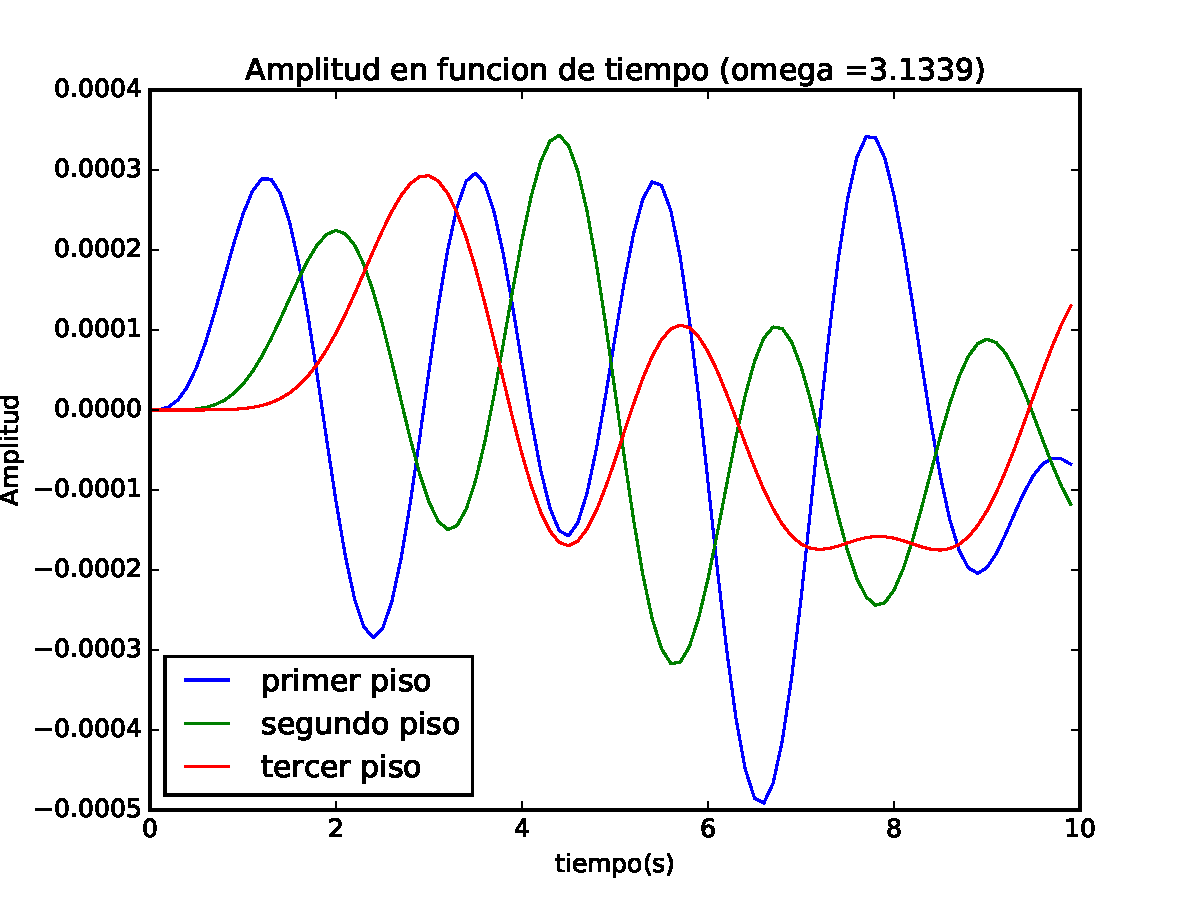
\includegraphics[width=10cm]{avst_o4.pdf} 
\end{center} 

El cuarto omega tiene un valor de 3.1339, este fue elegido porque estaba alejado de los picos que representan los modos normales, por esta razon vemos que los valores de las amplitudes en este caso son muy pequeños con respecto a los de las otras graficas. Aca uevamente vemos como el tercer piso es el menos afectado.


\end{document}
